\documentclass[11pt]{article}
\usepackage[lmargin=4.0cm, rmargin=4.0cm,tmargin=4cm,bmargin=4cm]{geometry}
\geometry{a4paper}                   % ... or a4paper or a5paper or ... 

\usepackage{graphicx}
\usepackage{amssymb}
\usepackage{amsmath}
\usepackage{epstopdf}
\usepackage{setspace}
\usepackage{hyperref}
\DeclareGraphicsRule{.tif}{png}{.png}{`convert #1 `dirname #1`/`basename #1 .tif`.png}


\renewcommand{\arraystretch}{1.5}

                       
\title{Phys1201 project: Circuit analysis with Python and SciPy}

\author{Buck Shlegeris (u5192430)}

\begin{document}

\maketitle

I created a set of Python programs which simulate arbitrary combinations of resistors, batteries, current sources, capacitors and inductors. Circuits are represented as a list of connections between nodes. The software can find resistances between arbitrary nodes, currents over all edges in a steady state system with no capacitors or inductors, and can find the evolution of current over time in a system with changing current, for example an RL circuit.\\

\subsection*{Representation of circuits}

The program takes a graph such as the following:\\

\texttt{[(0,1,[Resistor(1)]),\\
(0,1,[Resistor(1)]),\\
(1,0,[Battery(2)])]}\\

This is a simple circuit with two 1 Ohm resistors in parallel with a 2 volt battery.\\

Formally, the type of a circuit is a list of edges. An edge is a 3-tuple of start vertex, end vertex, and a list of components. Components are defined as Python objects with a variety of methods common across them. For example, the \texttt{getResistance} method returns 0 for a battery, and returns the resistance for a resistor.\\

Some components have more than one argument. For example, \texttt{Capacitor(1)} defines a capacitor with capacitance 1 Farad, while \texttt{Capacitor(1,3)} defines a capacitor with capacitance 1 Farad, but 3 Coulombs of initial charge on it.\\

\subsection*{Solving a steady system}

If we ignore inductors and capacitors, we can see how to find the steady state currents of a circuit using the node rule and voltage rule. The node rule is that the sum of currents going into a vertex equals the sum of currents going out of a vertex. The loop rule is that total power used across a loop equals the power given by the power sources along that loop.\\

These two rules generate a whole bunch of equations of the form $c_0I_0+c_1I_1+c_2I_2 ... = k$. In the case of the node rule we set $c_i$ to 1 if $I_i$ is a current which enters the node, -1 if $I_i$ is a current leaving the node, and 0 otherwise. $k$ is set to 0.\\

In the case of the loop rule, we set $c_i$ to the resistance across edge $i$ multiplied by the direction constant, which is 1 if the current is measured in the same direction as the loop goes across it, and -1 otherwise. The constant $k$ is set to\\

\begin{equation*}
k= \sum_{i\in I} d_i (v_i - c_i r_i )
\end{equation*}

where $d_i$ is the direction constant, $v_i$ is the voltage across the segment $i$, $c_i$ is the current generated by current sources along segment $i$, and $r_i$ is the resistance across segment $i$. The loops themselves are found with a simple recursive algorithm which traces along edges starting from a given vertex until it either gets back where it started, reaches a dead end, or reached the maximum loop length, which I'll discuss later.\\

These equations are concatenated to be the rows of an $m\times n$ matrix, where $m$ is the number of equations we have, and $n$ is the number of currents in the circuit. We are guaranteed to have more equations than currents, by simple graph theoretical arguments.\\

In this case, my system was obviously overdetermined, so I solved for currents using the linear least squares method, taken from the Fortran LAPACK library, which is provided as \texttt{scipy.linalg.lstsq} in the SciPy package.\\

This method allowed currents to be calculated in arbitrary systems of resistors, batteries, and current sources. Resistance between two points $a$ and $b$ on a circuit can be calculated by removing all current and voltage sources from the circuit, then adding a new edge $e$ between $a$ and $b$ with a $1V$ battery across it. The currents are then solved, and the resistance between $a$ and $b$ is equal to the reciprocal of the current along the edge $e$, directly from the definition $R=\frac{V}{I}$.\\

The first problem I tried to solve with my resistance methods was the knight's move problem, which I first saw on xkcd (\url{http://xkcd.com/356/}). I approximated this problem by looking at the resistance between two nodes a knight's move apart on various sized grids- I tried $10\times 10$, $15\times15$, and $18\times 18$ grids. These were prohibitively slow to calculate, as a result of the exponential growth in number of possible loops allowed as grid size increased. I added a global parameter which said that loops were to have a maximum size of six edges. This fixed the problem for that purpose, but could introduce weird bugs if particularly badly written circuits were considered.\footnote{For example, we can describe a simple circuit with a resistor and battery in series with five connectors in series between the battery and the resistor. This would look like \texttt{[(0,6,[Battery(1)]),(0,1,[]),(1,2,[]),(2,3,[]),(3,4,[]),(4,5,[]),(5,6,[Resistor(1)])]}. With a maximum loop length less than six, this circuit would be unsolvable. One obvious area of improvement to this program is trying to reduce circuits like that to simpler forms.}\\

This system has demonstrated success with a variety of problems, including finding the resistance between two opposite points on a cube of resistors finding the current in a variety of circuits with different components in parallel and series.\\

The initial current in a system with capacitors and inductors can be found by considering (initially chargeless) capacitors as closed switches and inductors as open switches. The final current can be found by considering capacitors as open switches and inductors as closed switches.\\

\subsection*{Components which vary smoothly over time}

Another class of components, in addition to static components previously dealt with, can be simulated at a given time step as a combination of simpler components. For example, if a capacitor has a charge $q$ stored on it, it generates a voltage $\frac{q}{C}$. This can be used to simulate the behaviour of a capacitor at a single instant, by treating it as a voltage. Once currents are calculated, the change in charge on the capacitor is given by the time step multiplied by the current. At the next time step, the new charge is used to calculate its effective voltage.\\

Capacitors can be accurately simulated this way because their behaviour approaches that of a voltage source as the time interval considered decreases. This method is actually just a method of integrating the equation $I(t)=-\int_0^t I dt$.\\

\begin{figure}
 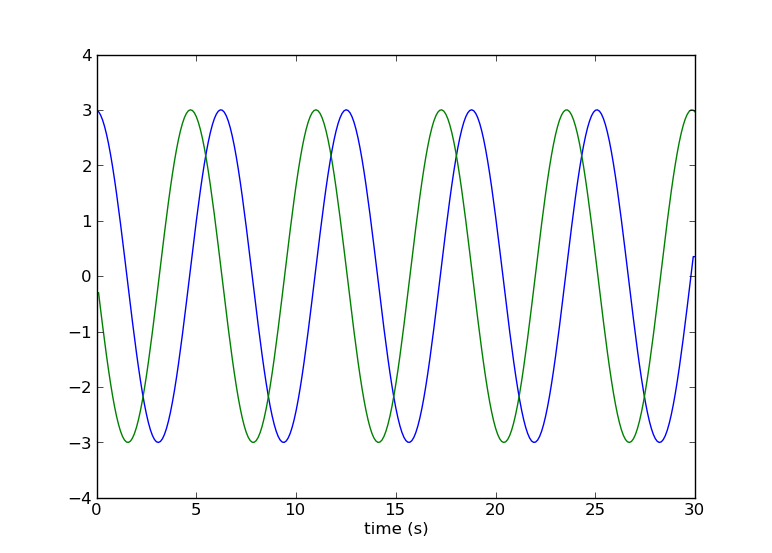
\includegraphics[scale=0.5]{LC_circuit.png}
\caption{An LC circuit, with capacitance 1 Farad and inductance 1 Henry, with an initial current of 3A. The blue line is current over time, and the green line is the charge in the capacitor.}
\end{figure}

Capacitors with dielectric breakdown are simulated by putting a cap on the amount of charge they can hold. When their charge is beyond this limit, they generate a voltage of 0, to simulate electrons breaking through the gap between the plates in the capacitor.\\

Non-ohmic resistors can be simulated by having the \texttt{getResistance} method pick a resistance based on the current which it saw last time step. This works to some extent.\\

\subsection*{Systems which vary jerkily over time}

Inductors are far more irritating to work with than capacitors, because the voltage across them is non-linear with respect to current over them\footnote{Obviously, inductors don't behave linearly with respect to current over them. What I mean by `non-linear' here is that there is no way to describe the inductor as some combination of Ohmic resistors, batteries, or current sources, which approaches the behaviour of the inductor as the time step approaches 0.}. It is impossible to simulate inductors usefully using the previous method (except for simply considering them open switches, over the very long term). As a result, a far more involved method using differential equations is needed.\\

The method for calculating currents is now just finding the change in currents as a function of the currents and the other properties of the circuit. We create the matrix equation $A\frac{d\textbf{I}}{dt}=B\textbf{I} + \textbf{x}$ and solve it for the change in currents vector $\frac{d\textbf{I}}{dt}$.\\

The node rule now provides a row vector for the matrix $A$ in the same way as before, a zero row for the matrix $B$, and a 0 entry in the vector $\textbf{x}$. The loop rule provides the same row vector for matrix $B$ as it did for the steady state system, uses the constant calculated in the same way as previously for an entry in \textbf{x}, and generates the row vector $a$ for matrix $A$ by setting $a_i$ to the inductance across edge $i$ multiplied by the direction constant.\\

Now, a linear least squares method is used to find the vector $\frac{d\textbf{I}}{dt}$. At this point, we have the vector $\frac{d\textbf{I}}{dt}$. I am attempting to find the current after some timestep. In lieu of cleverly integrating, I chose to simply multiply the rate of change of current and alter the initial current by that much. For example, if the rate of change of current were 0.1 and initial current were 1A, then the current after a timestep of 0.01 would be 1.001. This method approaches the correct value as timestep decreases.\\

The biggest problem with this method is that it now produces errors when loops around the circuit have too small an inductance relative to the time resolution of the simulation. Consider a simple circuit with a 1V battery, 1H inductor, and 1$\Omega$ resistor in series, where the circuit is closed at $t=0$. The rate of change of current at $t=0$ is 1. The current after one timestep of length $l$ is the initial current plus the time step multiplied by the derivative, which is just $l$ in this case. If $l<1$, then the system will correctly converge to a current of 1A. If $l=1$, then the system will abruptly jump to its final voltage after one timestep and stay there forever. If $2>l>1$, the current will initially rise above its correct final voltage, but will converge to the correct answer. If $l>2$, then the current diverges geometrically.\\

The obvious way of solving that problem is integrating more intelligently, even just by using SciPy's \texttt{odeint} module. This would be an obvious improvement to the project. However, this program would require a bit of rewriting to use that efficiently.

\section*{Conclusion}

The initial premise of this project was that all electrical components can be modelled for a given timestep as a combination of a resistor and a voltage source. This was correct for capacitors, but completely wrong for inductors. A more complicated method was found to simulate inductors.\\

Overall, I learned a lot from this project, mostly about electronics. I learned a variety of stuff about linear algebra and ODEs, much of which I didn't end up using in this project. One area which I did learn quite a bit about was how numerical linear algebra works- how QR decomposition is used instead of row reduction, and so on.\\

One thing I'm thinking of doing with this project is rewriting it so that it can simulate analogue signal processing components for sound effects- I could make cool amplifier simulations or something with it. That would probably require that I rewrite the whole thing in C, though, which would be a lot of effort.\\

\end{document}
